\documentclass{article}

\usepackage{multirow, graphicx, amsfonts, amsmath, amsthm, mathtools, tikz, tikz-qtree}

\addtolength{\oddsidemargin}{-.875in}
\addtolength{\evensidemargin}{-.375in}
\addtolength{\textwidth}{1.55in}

\addtolength{\topmargin}{-.375in}
\addtolength{\textheight}{1.75in}

\newcommand\cperm[2][^n]{\prescript{#1\mkern-2.5mu}{}P_{#2}}
\newcommand\ccomb[2][^n]{\prescript{#1\mkern-0.5mu}{}C_{#2}}

\newtheorem{theorem}{Theorem}[section]
\newtheorem{corollary}{Corollary}[theorem]
\newtheorem{lemma}[theorem]{Lemma}

\newcommand{\bipgraph}[2]{
    \begin{tikzpicture}[every node/.style={circle,draw}]
		\foreach \xitem in {1,2,...,#1}
		{
			% first set
			\node at (0,\xitem) (a\xitem) {};
			% second set
			\node at (2,\xitem) (b\xitem) {};   
		}

		% connections
		\foreach \x [count=\xi] in {#2}
		{
			\foreach \tritem in \x
			\draw(a\xi) -- (b\tritem);
		}
    \end{tikzpicture}  
}

\begin{document}

	\begin{center}
		\LARGE{AGT Summative Assignment -- Individual Component Report}\\[0.1cm]
		\Large{wcrr51}\\[0.1cm]
		2021\\[0.5cm]
	\end{center}

	\begin{enumerate}

		\item[\textbf{Exercise 1.}]   %%%%%%%  11 MARKS  %%%%%%% 
		
Consider the following instance of the load balancing game where the number of tasks is equal to the number of machines, and in particular we have:
\begin{itemize}
    \item $m$ identical machines $M_1, M_2, \dots, M_m$ (all of speed 1),
    \item $m$ identical tasks $w_1 = w_2 = \dots = w_m = 1$.
\end{itemize}
Consider also the mixed strategy profile $A$ where each of the tasks is assigned to all machines equiprobably (i.e. with probability $1/m$).
\begin{enumerate}
    \item[(a)] Calculate the ratio $cost(A)/cost(OPT)$ in the special case where $m=2$.  \hfill{\bf [3 marks]}\smallskip

    Trivially, makespans of $1$ and $2$ have $2$ assignments each.
    Hence, for $m = 2$, there are a total of $2^2 = 4$ possible assignments.
    These assignments are shown in Table~\ref{tab:ex1a}.

    \begin{table}[ht!]
        \centering
        \begin{tabular}{cccc}
          & $M_1$ & $M_2$ & Makespan \\ \hline
        1 & 1, 2  & -     & 2        \\
        2 & -     & 1, 2  & 2        \\
        3 & 1     & 2     & 1        \\
        4 & 2     & 1     & 1
        \end{tabular}
        \caption{Task-machine assignments for $m = 2$ in Exercise 1}
        \label{tab:ex1a}
    \end{table}

    From this, $cost(A)$ can be calculated with
    \begin{equation}
        cost(A) = E[cost(B)] = \sum_{i = 1}^{m} P(cost(B) = i) \cdot i
        \label{eq:ex1-cost-a}
    \end{equation}

    Since there is capacity for one machine per task, and this would be the optimal assignment for any positive $m$, hence, it holds true that
    \begin{equation}
        \forall{m} > 0, cost(OPT) = 1
        \label{eq:ex1-opt-cost}
    \end{equation}

    For $m = 2$, using~\eqref{eq:ex1-cost-a}, $cost(A) = E[cost(B)] = \frac{1}{4} (1 \cdot 2 + 2 \cdot 2) = \frac{6}{4} = \frac{3}{2} = 1.5$.

    Combining this with~\eqref{eq:ex1-opt-cost}, the ratio $cost(A)/cost(OPT)$ for $m = 2$ is $\frac{3}{2} / 1 = \frac{3}{2} = 1.5$

    \item[(b)] Calculate the ratio $cost(A)/cost(OPT)$ in the special case where $m=3$.  \hfill{\bf [3 marks]}\smallskip

    For a makespan of $1$, there are $\cperm[3]{3} = 3! = 6$ assignments, for $2$, there are $3 \cdot \cperm[3]{2} = 18$ assignments and for $3$, there are trivially $3$ assignments.
    Hence, for $m = 3$ there are a total of $3^3 = 27$ possible assignments.
    These assignments are shown in Table~\ref{tab:ex1b}.

    \begin{table}[ht!]
        \centering
        \begin{tabular}{ccccc}
           & $M_1$   & $M_2$   & $M_3$   & Makespan \\ \hline
        1  & 1, 2, 3 & -       & -       & 3        \\
        2  & -       & 1, 2, 3 & -       & 3        \\
        3  & -       & -       & 1, 2, 3 & 3        \\
        4  & 1       & 2, 3    & -       & 2        \\
        5  & 1       & -       & 2, 3    & 2        \\
        6  & -       & 1       & 2, 3    & 2        \\
        7  & 2, 3    & 1       & -       & 2        \\
        8  & 2, 3    & -       & 1       & 2        \\
        9  & -       & 2, 3    & 1       & 2        \\
        10 & 2       & 1, 3    & -       & 2        \\
        11 & 2       & -       & 1, 3    & 2        \\
        12 & -       & 2       & 1, 3    & 2        \\
        13 & 1, 3    & 2       & -       & 2        \\
        14 & 1, 3    & -       & 2       & 2        \\
        15 & -       & 1, 3    & 2       & 2        \\
        16 & 3       & 1, 2    & -       & 2        \\
        17 & 3       & -       & 1, 2    & 2        \\
        18 & -       & 3       & 1, 2    & 2        \\
        19 & 1, 2    & 3       & -       & 2        \\
        20 & 1, 2    & -       & 3       & 2        \\
        21 & -       & 1, 2    & 3       & 2        \\
        22 & 1       & 2       & 3       & 1        \\
        23 & 2       & 1       & 3       & 1        \\
        24 & 2       & 3       & 1       & 1        \\
        25 & 3       & 2       & 1       & 1        \\
        26 & 3       & 1       & 2       & 1        \\
        27 & 1       & 3       & 2       & 1
        \end{tabular}
        \caption{Task-machine assignments for $m = 3$ in Exercise 1}
        \label{tab:ex1b}
    \end{table}

    For $m = 3$, using~\eqref{eq:ex1-cost-a}, $cost(A) = E[cost(B)] = \frac{1}{27} (1 \cdot 3 + 2 \cdot 18 + 3 \cdot 3) = \frac{51}{27} = \frac{17}{9} \approx 1.89$.
    Combining this with~\eqref{eq:ex1-opt-cost}, the ratio $cost(A)/cost(OPT)$ for $m = 3$ is $\frac{17}{9} / 1 = \frac{17}{9} \approx 1.89$

    \item[(c)] Discuss what this ratio is for arbitrary $m$. What does this imply about the Price of Anarchy on identical machines for mixed Nash equilibria?  \hfill{\bf [5 marks]}\smallskip

    As~\eqref{eq:ex1-opt-cost} holds true for all $m > 0$, the denominator of the $cost(A)/cost(OPT)$ ratio is always one.
    This means that, for this instance of the load balancing game, $cost(A)$ determines what the fraction will be.

    There are $m^m$ possible task to machine assignments, distributed over $m$ makespan values (from $1$ to $m$).
    Through equiprobable assignment of tasks to machines, let $p_i$ be the probability of an assignment with makespan $i = 1, 2, \ldots, m$ where $\sum_{i = 1}^{m}{p_i} = 1$, given by 
    \[
        p_i = \frac{c_i}{m^m}
    \]
    Where $c_i$ is the number of combinations of task to machine assignments with a makespan $i$ (for example, for $m = 3$, and makespans $i = 1, 2, 3$, $c_1 = 6, c_2 = 18, c_3 = 3$, and hence $p_1 = \frac{6}{27} = \frac{2}{9}, p_2 = \frac{2}{3}, p_3 = \frac{1}{9}$).

    This would, for arbitrary $m$, yield
    \[
        cost(A) = \sum_{i = 1}^{m} \frac{i \cdot c_i}{m^m}
    \]
    Note that $\sum_{i = 1}^{m}{c_i} = \implies \forall i > 1, c_i < m^m$, this means that $cost(A)$ is bound to lie within the makespan distribution (between $1$ and $m$), implying the Price of Anarchy for identical machines is relatively low.
    Furthermore, this is backed up by a known theorem (Slide 50 of Week 5) which states that $\frac{cost(Q)}{cost(OPT)} = O\left(\frac{\log{m}}{\log{\log{m}}}\right) => \texttt{PoA} = \Theta \left(\frac{\log{m}}{\log{\log{m}}}\right)$ for any Nash equilibrium strategy profile $Q$ on identical machines.
    Because of this, it also implies that the price of anarchy for mixed Nash equilibria on identical machines is quite small, and hence, provides a lower bound on the price of anarchy across all load balancing games.

\end{enumerate}
\vspace*{0.8cm}

		\newpage


		\item[\textbf{Exercise 2.}]   %%%%%%%  10 MARKS  %%%%%%% 
		
We consider a second-price sealed-bid auction where there are $n$ bidders who bid as follows:
\begin{itemize}
    \item Bidders 1 up to $n - 1$ bid either 1 dollar or $r > 1$ dollars equiprobably and
    independently of the rest.
    \item Bidder $n$ bids $h$ dollars, where $h > r$.
\end{itemize}
The seller's expected revenue $R$ is the expectation of the second highest value. 
\begin{itemize}
    \item[(a)] What is the value that $R$ is approaching when $n$ is very large? \hfill{\bf [1 marks]}\smallskip

    For large $n$, $R$ approaches $r$.

    \item[(b)] Justify your answer by taking the limit. \hfill{\bf [9 marks]}\smallskip

    Trivially and by the definition, $R$ must be less than $h$.

    Let $X$ be a binomially distributed random variable representing the number of times $r$ is chosen (instead of $1$) from a set of $n - 1$ independent trials (representing independent bidders $1$ to $n - 1$), each of probability $\frac{1}{2}$.
    \begin{equation}
        X \sim B{ \left( n - 1, \frac{1}{2} \right) }
    \end{equation}

    $P(X = 0)$ is the probability that $r$ is chosen $0$ times across the $n - 1$ independent trials.
    \begin{equation}
        \begin{split}
            & P(X = 0) = \ccomb[n - 1]{0} \cdot \frac{1}{2}^0 \cdot \frac{1}{2}^{(n - 1) - 0}
            = \frac{1}{2}^{n - 1} = 2^{-(n - 1)} = 2^{1 - n} = 2 \cdot 2^{-n} \\
            & \implies \lim_{n -> \infty}{P(X = 0)} = \lim_{n -> \infty}{ \left( 2 \cdot 2^{-n} \right) }
            = 2 \cdot \lim_{n -> \infty}{2^{-n}} = 2 \cdot 0 = 0
        \end{split}
    \end{equation}
    This means that as $n$ increases, the probability of $r$ not being chosen approaches zero.
    Hence, the larger the value of $n$, the more likely an $r$ will be chosen, and thus the more likely $R = r$.

\end{itemize}

		\newpage


		\item[\textbf{Exercise 3.}]   %%%%%%%  15 MARKS  %%%%%%% 
		
Mary and Alice are buying items for Sunday lunch. Mary buys either chicken $(C)$ or beef $(B)$ for the main course and Alice buys either juice $(J)$ 
or wine $(W)$. Both people prefer wine with beef and juice with chicken. The opposite alternatives are equally displeasing.
However, Mary prefers beef over chicken, while Alice prefers chicken over beef.

We assume that Mary buys first and then tells Alice what she bought,
so when Alice makes her decision, she knows if the main course is beef or chicken.

\begin{enumerate}
    \item[(a)] Express the above preferences as payoffs by using numbers\\
    (e.g. $u_M(B, W) = 2$, $u_A(B, W) = \ldots$  etc.) \hfill{\bf [2 marks]}\smallskip

    As Mary prefers $B$ over $C$, and Alice prefers $C$ over $B$, $u_M(B, W) > u_A(B, W)$ and $u_M(C, J) < u_A(C, J)$.
    As both prefer $B$ with $W$ and $C$ with $J$, $u_i(B, W) > 0, u_i(C, J) > 0 : i \in \{M, A\}$
    As both are equally displeased by $B$ with $J$ and $C$ with $W$, $u_i(B, J) = u_i(C, W), u_i(B, J) < u_i(B, W), u_i(C, W) < u_i(B, J) : i \in \{M, A\}$

    The following assignment satisfies these constraints:
    \begin{equation}
        \begin{split}
            u_M(B, W) = 2, u_A(B, W) = 1, \\
            u_M(B, J) = 0, u_A(B, J) = 0, \\
            u_M(C, W) = 0, u_A(C, W) = 0, \\
            u_M(C, J) = 1, u_A(C, J) = 2
        \end{split}
    \end{equation}

    \item[(b)] Write down a bimatrix game with Mary as the row player and Alice as the column player, using your chosen payoffs. \hfill{\bf [4 marks]}\smallskip

    \begin{table}[ht!]
        \centering
        \begin{tabular}{lc|cl|cl|}
        \cline{3-6}
         &  & \multicolumn{4}{c|}{Alice}                      \\ \cline{3-6} 
         &  & \multicolumn{2}{c|}{J} & \multicolumn{2}{c|}{W} \\ \hline
        \multicolumn{1}{|c|}{\multirow{2}{*}{Mary}} & C                      & 1                     & \multicolumn{1}{c|}{2} & 0                     & \multicolumn{1}{c|}{0} \\ \cline{2-6} 
        \multicolumn{1}{|c|}{}                      & \multicolumn{1}{l|}{B} & \multicolumn{1}{l}{0} & 0                      & \multicolumn{1}{l}{2} & 1                      \\ \hline
        \end{tabular}
        \caption{Bimatrix game representation of the scenario in Exercise 3}
        \label{tab:ex3b}
    \end{table}

    \item[(c)] Write down a game tree representing this game as an extended game.  \hfill{\bf [4 marks]}\smallskip

    As Mary buys first, she is at the root of the tree, the two outward edges represent the choice between $B$ and $C$.
    Whether $B$ or $C$ is chosen, Alice is the next node, these each have two edges representing the choice between $W$ and $J$.
    Finally, the leaves represent the payoffs for each player from the corresponding actions taken from the root to the leaf.

    \hfil
    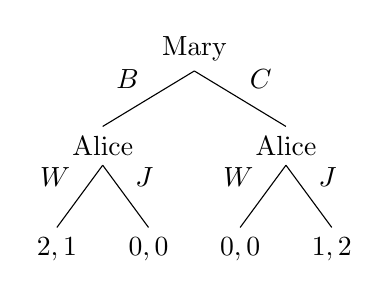
\begin{tikzpicture}[level distance=36pt,sibling distance=12pt]
    \Tree [.Mary
        \edge node[auto=right]{$B$};
        [.Alice
        \edge node[auto=right]{$W$}; $2,1$
        \edge node[auto=left]{$J$}; $0,0$ ]
        \edge node[auto=left]{$C$};
        [.Alice
        \edge node[auto=right]{$W$}; $0,0$
        \edge node[auto=left]{$J$}; $1,2$ ]
    ]
    \end{tikzpicture}
    \hfil

    \item[(d)] Find a solution for the extended game using backward induction.\\Describe your steps.  \hfill{\bf [5 marks]}\smallskip

    For this solution, an edge with a solid line represents the action that is chosen. 

    Firstly consider the left subgraph (taking action $B$), Alice may either choose $W$ with reward $1$ or $J$ with reward $0$.
    As $1 > 0$, Alice chooses $W$ and her node takes the payoff value $2,1$.

    \hfil
    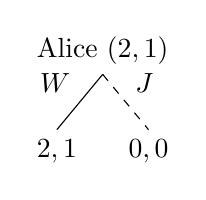
\begin{tikzpicture}[level distance=36pt,sibling distance=12pt]
    \Tree [.\text{Alice ($2,1$)}
        \edge node[auto=right]{$W$}; $2,1$
        \edge[dashed] node[auto=left]{$J$}; $0,0$
    ]
    \end{tikzpicture}
    \hfil

    Next, return to the root and consider its right subgraph (taking action $C$), Alice may either choose $W$ with reward $0$ or $J$ with reward $2$.
    As $0 < 2$, Alice chooses $W$ and her node takes the payoff value $1,2$.

    \hfil
    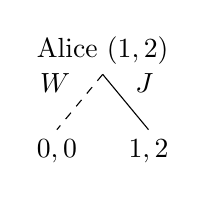
\begin{tikzpicture}[level distance=36pt,sibling distance=12pt]
    \Tree [.\text{Alice ($1,2$)}
        \edge[dashed] node[auto=right]{$W$}; $0,0$
        \edge node[auto=left]{$J$}; $1,2$
    ]
    \end{tikzpicture}
    \hfil

    Finally, consider the root. Mary may either choose $B$ with reward $2$ or $C$ with reward $1$.
    As $2 > 1$, Alice chooses $B$.

    \hfil
    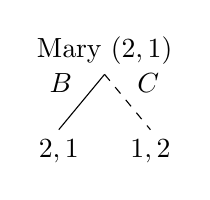
\begin{tikzpicture}[level distance=36pt,sibling distance=12pt]
    \Tree [.\text{Mary ($2,1$)}
        \edge node[auto=right]{$B$}; $2,1$
        \edge[dashed] node[auto=left]{$C$}; $1,2$
    ]
    \end{tikzpicture}
    \hfil

    The full annotated graph is as follows.

    \hfil
    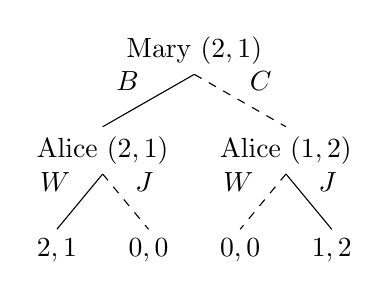
\begin{tikzpicture}[level distance=36pt,sibling distance=12pt]
    \Tree [.\text{Mary ($2,1$)}
        \edge node[auto=right]{$B$};
        [.\text{Alice ($2,1$)}
        \edge node[auto=right]{$W$}; $2,1$
        \edge[dashed] node[auto=left]{$J$}; $0,0$ ]
        \edge[dashed] node[auto=left]{$C$};
        [.\text{Alice ($1,2$)}
        \edge[dashed] node[auto=right]{$W$}; $0,0$
        \edge node[auto=left]{$J$}; $1,2$ ]
    ]
    \end{tikzpicture}
    \hfil

    Hence, by backwards induction, Mary gets a higher payoff than Alice and they have Beef with Wine for Sunday lunch.

\end{enumerate}
\vspace*{0.8cm}

		\newpage


		\item[\textbf{Exercise 4.}]   %%%%%%%  12 MARKS  %%%%%%% 
		
We consider a (matching) market of $k$ sellers and $k$ buyers, where $k$ is an integer, $k>0$. 
Each seller sells an item and the prices of the items are initially all zero. Buyer $i$ has valuation $k-i+1$ for the first item and valuation $0$ for every other item, as shown in the following diagram.

\vspace*{0.5cm}
\begin{tabular}{c r c c c}
    Buyers & \multicolumn{4}{c}{Valuations (for items $1$ to $k$)} \\
    \hline
    $x_1$ & $k,$ & $0,$ & $\ldots,$ & $0$ \\
    $x_2$ & $k-1,$ & $0,$ & $\ldots,$ & $0$ \\
    $\vdots$ & & & $\vdots$ \\
    $x_k$ & $1,$ & $0,$ & $\ldots,$ & $0$ \\
\end{tabular}

\noindent The sellers find the market-clearing prices using the procedure discussed in the lectures.
\begin{enumerate}
    \item[(a)] What are the prices of the sellers' items ($1^{st}$ item, $2^{nd}$ item, \ldots, $k^{th}$ item) when the market clears? Which buyer gets the $1^{st}$ item and at what price?  \hfill{\bf [3 marks]}\smallskip

    The $1^{st}$ item is sold at a price of $k - 1$.
    The $2^{nd}$ to $k^{th}$ items are sold at a price of $0$.

    Buyer $x_1$ gets the $1^{st}$ item at a price of $k - 1$.

    \item[(b)] Justify your answers to (a).  \hfill{\bf [6 marks]}\smallskip

    Let Algorithm 1 be the procedure for finding market-clearing prices as shown in the lectures and $x_{j,i}$ be the valuation of item $i$ by buyer $j$.

    \begin{theorem}
        The matching market in this case results in the market-clearing prices $(k - 1, 0, \dots, 0)$ for items $1, 2, ..., k$.
    \end{theorem}

    \begin{proof}
        Using induction.

        \underline{Base case ($k = 1$)}:
    
        Applying Algorithm 1, the $1^{st}$ seller's price $p_1$ is initially $0$.
        This trivially produces the following preferred-seller graph since buyer $x_1$ values the item at $1$, giving them a positive payoff of $x_{1,1} - p_1 = 1 - 0 = 1$.

        \hfil
        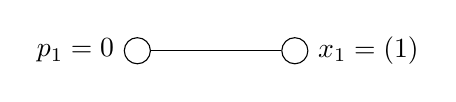
\begin{tikzpicture}[main/.style={circle,draw}]
            \node[main, label={left:$p_1 = 0$}] at (0, 2) (p1) {};

            \node[main, label={right:$x_1 = (1)$}] at (2, 2) (x1) {};

            \draw(p1) -- (x1);
        \end{tikzpicture}
        \hfil

        This is clearly a perfect bipartite matching, hence, for $k = 1$, the theorem holds.

        Next, consider $k = n$ for a positive integer $n$.

        In this case, trivially, any buyer 

        \begin{lemma}
            Any complete bi-partite graph $K_{n, n}, n > 0$ has a perfect matching.
        \end{lemma}
        \begin{proof}
            Trivial, connect left node $i$ to right node $i$ for all $1 \leq i \leq n$.
        \end{proof}

        \hfil
        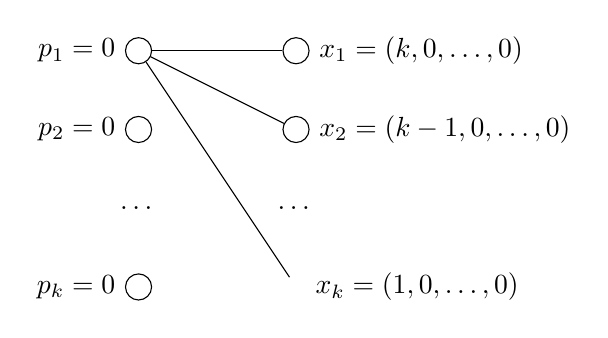
\begin{tikzpicture}[main/.style={circle,draw}]
            \node[main, label={left:$p_1 = 0$}] at (0, 2) (p1) {};
            \node[main, label={left:$p_2 = 0$}] (p2) [below of=p1] {};

            \node (pDots) [below of=p2] {\dots};

            \node[main, label={left:$p_k = 0$}] (pk) [below of=pDots] {};

            \node[main, label={right:$x_1 = (k, 0, \dots, 0)$}] at (2, 2) (x1) {};
            \node[main, label={right:$x_2 = (k - 1, 0, \dots, 0)$}] (x2) [below of=x1] {};

            \node (xDots) [below of=x2] {\dots};

            \node[label={right:$x_k = (1, 0, \dots, 0)$}] (xk) [below of=xDots] {};

            \draw(p1) -- (x1);
            \draw(p1) -- (x2);
            \draw(p1) -- (xk);
        \end{tikzpicture}
        \hfil

        Trivially, a single edge from item 1 to 
        
        \begin{corollary}
            Removing the vertices for seller $1$ and buyer $x_1$ from the preferred-seller graph yields the complete bipartite graph $K_{k - 1,k - 1}$
        \end{corollary}
    \end{proof}

    \item[(c)] Which kind of auction does the construction of market-clearing prices procedure implement in this case?  \hfill{\bf [3 marks]}\smallskip

    As the winner of item $1$ is the buyer ($x_1$ in this case) who values it the highest.
    They pay the valuation of item $1$ by the second highest buyer ($k - 1$ in this case). 
    Thus, the construction of market-clearing prices implements a second-price (Vickrey) auction for item 1 in this case.

\end{enumerate}


	\end{enumerate}

\end{document}